\documentclass[a4paper,pdftex,oneside,10pt,mathsans]{scrartcl} %,fleqn

% Wir geben alles im UTF-8 Zeichensatz ein (alles andere ist Unfug!)
\usepackage[T1]{fontenc}
\usepackage[utf8]{inputenc}
\usepackage{ngerman}

\newcommand{\Autoren}{\href{buchegger.uni@gmail.com}{Philipp Buchegger}}

\newcommand{\Gruppe}{Studienarbeit}
\newcommand{\Thema}{CPT Uni Tübingen}
\newcommand{\Titel}{Scheibendynamik in Binärsternsystemen mit FARGO}
\newcommand{\Datum}{Tübingen, den 26. Juli 2010}
\newcommand{\Schluesselwoerter}{}


\usepackage{ae}

% Wir verwenden die neue deutsche Rechtschreibung (wir versuchen es zumindest ^^)
\usepackage{ngerman}
\usepackage[english,ngerman]{babel}

% Wir m�hten Grafiken verwenden und diese sollen als Ausgabetreiber pdfTex verwenden
\usepackage[pdftex]{graphicx}

% Keine Papierverschwendung wie es bei Tex-Standard blich ist
\usepackage[bottom=30mm,top=25mm,inner=20mm,outer=20mm,marginparwidth=15mm,marginparsep=3mm,headsep=10mm]{geometry}

% Die zus�zlichen AMS-Mathepakete, und sch�ere Integralgrenzen
\usepackage[intlimits]{amsmath}
\usepackage{amsthm}
\usepackage{amsopn}
\usepackage{amscd}
\usepackage{amsfonts}
\usepackage{amssymb}
%\usepackage{mathrsfs}

% Einheitenbefehle \unit und \unitfrac
\usepackage{units}

% Sch�ere und flexiblere Kopfzeilen
\usepackage{fancyhdr}

% Ab und zu m�hten wir Seiten im Querformat einbauen
\usepackage{pdflscape}

% Vorschau PDFs erstellen
\usepackage{thumbpdf}

% Type1-Fonts (damit die PDFs nicht so verpixeln)
% Folgende Pakete sollten deshalb installiert sein:
% Font-Packages: CTAN: fonts/cmbright/, CTAN: fonts/ps-type1/cm-super/, CTAN: fonts/ps-type1/hfbright/
\usepackage{type1cm}

% Komplette PDFs (oder Seiten daraus) importieren
\usepackage{pdfpages}

% If-Abfragen erm�lichen
\usepackage{ifthen}

% Quellcodes sch� darstellen
\usepackage{verbatim}

% Erweitere Quellcodedarstellung
\usepackage{listings}

% Verschiedene Pakete (was machten die nochmals?)
\usepackage{titling}
\usepackage{textcomp}
\usepackage{nonfloat}
\usepackage{booktabs}

% Erweitere Aufz�lungen
\usepackage{eqlist}
\usepackage{paralist}

% Farbuntersttzung
\usepackage{color}

% PDF spezifische Funktionen
\usepackage[a4paper,breaklinks,unicode,colorlinks,linktocpage,pdftex,linkcolor=blue,urlcolor=blue,backref,pagebackref,bookmarks,bookmarksnumbered]{hyperref}

% dsfont
\usepackage{multicol,wasysym,expdlist}

% kleine Layoutfehler fixen
\usepackage{ellipsis,fixltx2e,mparhack}

\usepackage{microtype}

% absolute Textpositionierung
\usepackage{textpos}

% Indexerstellung
\usepackage{makeidx}
\usepackage{booktabs}

% Immer Serifenlos schreiben
\renewcommand{\familydefault}{\sfdefault}

% Abs�ze nicht einrcken
\setlength{\parindent}{0em}

% Titel, Autor, Datum konfigurieren (fr Titelseite)
\title{ \textbf{\Titel} \\ \Thema}
\ifthenelse{ \equal{\Gruppe}{} }{ \author{\Autoren} }{ \author{\Autoren \\ \Gruppe}}
\date{\Datum}

% PDF Informationen
\hypersetup{
  pdftitle=\Titel,
  pdfsubject=\Thema,
  pdfauthor=\Autoren,
  pdfkeywords=\Schluesselwoerter,
  pdfcreator={LaTeX},
  pdfproducer={LaTeX}
  %pdfpagemode=None
  %pdfpagelayout=Singlepage  (keine Lesezeichen)
}

\fancypagestyle{plain}{%
}

% C++ Layout fuer Quellcodes importieren
\lstloadlanguages{c++}

\begin{document}
\definecolor{Gray}{gray}{0.5}

% Farben und Quellcodedefinitionen fr die sch�e Darstellung von LISP/Scheme
\definecolor{darkblue}{rgb}{0,0,.6}
\definecolor{darkred}{rgb}{.6,0,0}
\definecolor{darkgreen}{rgb}{0,.6,0}
\definecolor{red}{rgb}{.98,0,0}
%
\lstset{
  numbers=left,
  numberblanklines=false,
  showspaces=false,
  showstringspaces=false,
  numberstyle=\tiny,
  language=C++,
  inputencoding=utf8,
  extendedchars=true,
  basicstyle=\ttfamily,
  commentstyle=\itshape\color{Gray},
  keywordstyle=\bfseries\color{darkblue},
  directivestyle=\color{darkgreen},
  stringstyle=\color{darkred},
  breaklines,
  postbreak=\space,
  breakindent=5pt,
  tabsize=8}

% normalerweise mit Buchstaben a), b) aufz�len
\renewcommand{\labelenumi}{\alph{enumi})}

% keine Nummerierung der �erschriften
\setcounter{secnumdepth}{0}

% etwas kleinere Formelabst�de
\setlength{\jot}{6pt}

% Seitenlayout mit Kopfzeilen definieren
\pagestyle{fancy}
\rhead{\today}
\chead{}
\lhead{\textbf{\Titel} \\ \Thema}
\lfoot{\Autoren}
\cfoot{}
\rfoot{\thepage}
\renewcommand{\headrulewidth}{0.4pt}
\renewcommand{\footrulewidth}{0.4pt}
\renewcommand{\headheight}{25.pt}

% Titelseite erstellen
\maketitle

% Und etwas Platz darunter lassen
\vspace{1em}

\setlength{\baselineskip}{1.25\baselineskip}
\setlength{\parskip}{\baselineskip}
\setcounter{secnumdepth}{3}
\setcounter{tocdepth}{3}
\setlength{\plitemsep}{0.3\baselineskip}

\setlength{\abovedisplayskip}{0.5\baselineskip}
\setlength{\abovedisplayshortskip}{0pt}
\setlength{\belowdisplayskip}{0.5\baselineskip}
\setlength{\belowdisplayshortskip}{0.5\baselineskip}

\newcommand{\super}[1]{\ensuremath{^{\textrm{#1}}}}
\newcommand{\sub}[1]{\ensuremath{_{\textnormal{#1}}}}

\newcommand{\e}{\mathrm e}

\tableofcontents 
\section{Einleitung}
Gibt es noch anderes Leben im Universum? Getrieben von dieser Frage suchten Astrophysiker nach erdähnlichen Planeten, welche um einen Stern ähnlich der Sonne kreisen. Dies ist eine geringe Voraussetzung, welche auch noch recht offen formuliert ist. Trotzdem ist selbst diese Suche keine Einfache: 
Die erste bestätigte Entdeckung eines Exoplaneten war erst im Jahr 1988 von Bruce Campbell, G. A. H. Walker, und S. Yang \cite{campbellwalkeryang}. Dieser Exoplanet ist im System $\gamma$ Cephei, welches wir später genauer untersuchen. 
Mit der Entdeckung des ersten Exoplaneten in einem sonnenähnlichen System 1995 \cite{mayorqueloz} begann die Goldgräberstimmung bei vielen Astrophysikern, andere Exoplaneten zu finden. Mittlerweile gibt es 464 Exoplaneten (Stand 16. Juli 2010).
Wie entstehen diese? Da Planetenentstehung selbst von einem Planetesimal ausgehend ein sehr langwieriger Prozess von mehreren Hunderttausend bis Millionen Jahren ist, sind Beobachtungen der Entwicklung nicht möglich. Desweiteren wurden bisher zu wenig Exoplaneten insgesamt gefunden, um daraus weitere Erkenntnisse zu ziehen.


Wir betrachten jetzt das Modell der turbulenten Akkretionsscheibe. 


Eine Akkretionsscheibe ist eine um ein zentrales Objekt rotierende Scheibe, die Materie in Richtung des Zentrums transportiert, also akkretiert. Sie kann aus atomarem Gas oder Staub bestehen. In dieser Studienarbeit wird die Störung der Scheibe durch einen Binärstern hervorgerufen. Die Simulation des Modells wird mit F. Massets FARGO-Code, modifiziert von C. Baruteau und T. Müller durchgeführt.

Ziel ist es, eine Studie über die Dynamik von zweidimensionalen Scheiben zu machen, die in der orbitalen Ebene, welche von dem Primärstern und Sekundärstern aufgespannt wird, liegt.

Wir gehen von einer anfangs ungestörten Scheibe aus, die nur durch den Binärstern gestört wird.



\subsection{Nachweismethoden von Exoplaneten}
Bislang konnte man die meisten Exoplaneten nicht direkt nachweisen, dies liegt an den grossen Entfernungen und den damit verbundenen geringen Helligkeitsintensitäten, sowie dem schlechten Auflösungsvermögen. Es gibt aber auch einige wenige Ausnahmen: Am 10. September 2004 wurde der erste Exoplanet direkt aufgenommen: der 225 Lichtjahre entfernte Braune Zwerg 2M1207.
Dafür gibt es einige indirekte Methoden:
\begin{itemize}
\item Transitmethode oder Durchgangsmethode: Diese Methode lässt sich nur anwenden, wenn die Umlaufbahn des Planeten so liegt, dass der Planet aus der Sicht des Betrachters genau vor dem Stern vorbeizieht. Diese periodische Absenkung der Helligkeit lässt sich mit hochpräziser Photometrie nachweisen. 
\item Radialgeschwindigkeitsmethode: Falls man von der Erde aus nicht genau senkrecht auf die Bahn des Sterns schaut, so bewegt sich der Stern periodisch vor und zurück. Anhand von Blau- und Rotverschiebung durch den Dopplereffekt und bekannter Sternmasse lässt sich so eine Untergrenze für die Planetenmasse berechnen. Mit dieser Methode wurden bisher die meisten Exoplaneten nachgewiesen.
\item Astrometrische Methode: Seit Mitte des 20. Jhd. wurde mit dieser Methode nach Exoplaneten gesucht, doch waren die Beobachtungen zu ungenau, um Exoplaneten zu entdecken. Man betrachtet die Bewegung des Sterns um den gemeinsamen Schwerpunkt des Sterns und der Planeten.
\item Gravitational microlensing-Methode: Diese indirekte Methode nutzt Effekte des Sternenhintergrundes.
\item Berechnung nach gestörter Planetenbahn: Eine indirekte Methode, die auf der Beobachtung bereits bekannter Exoplaneten beruht. Mittels Computersimulationen wird die Existenz eines Exoplaneten anhand von Störungen in der Bahn des benachbarten Planeten gezeigt.
\end{itemize}


\section{FARGO}
FARGO \cite{FARGO} ist ein in C bzw. C++ geschriebener Hydrocode, welcher in einem 2-dimensionalen Polargitter die Entwicklung von Akkretionsscheiben berechnen kann. FARGO hat folgende Features:
\begin{itemize}
\item löst die Navier-Stokes-Gleichung und Kontinuitätsgleichung für eine Keplersche Scheibe um den Zentralstern, sowie für umlaufende Planeten
\item Isotherme Zustandsgleichung mit frei wählbarer Temperatur oder Schallgeschwindigkeit
\item 2D Polargitter Hydrocode
\item van Leer upwind Algorithmus auf einem staggered mesh
\item frei wählbare Anzahl an Planeten bzw. jetzt Sternen
\item FARGO-Algorithmus (Fast Advection in Rotating Gaseous Objects)
\item OpenMP und MPI parallelisiert
\end{itemize}
Wenn Akkretionsscheiben von Binärsternen gestört werden, ist das ein sehr langwieriger Prozess, wenn der Binärstern nicht gerade sehr nahe an der Scheibe ist, oder seine Umlaufbahn eine hohe Exzentrizität hat. Das heißt, der Code muss schnell laufen, da wir die Entwicklung der Akkretionsscheibe über mehrere Tausend Jahre betrachten. Die Parallelisierung in OpenMP und MPI ist hier ein entscheidender Faktor: FARGO teilt das Gitter in mehrere Gitter-Ringe auf. Jeder Prozessor berechnet so nur einen kleinen Teil des Problems. Die Kommunikation der Gitter untereinander folgt über 5 überlapp-Zellen an den zwei Rändern. Das zeigt aber auch, da man diese Überlapp-Zellen immer mehrfach berechnen muss, dass man mit einem Computer mit mehreren Prozessoren nicht zwangsläufig schneller zu einem Ergebnis kommt, sondern "nur" in der selben Zeit in einer höheren Auflösung rechnen kann.

Für ein 300x300 Gitter zum Beispiel macht es  keinen Sinn, mit mehr als 16 Prozessoren zu rechnen, da jeder Ring zu seinen 19 Radialzellen nocheinmal 10 überlapp-Zellen dazubekommt. Insgesamt sind also mit 16 Prozessoren 464 Radialzellen zu berechnen. Wenn man das ganze mit 8 Prozessoren berechnet hätte, wären es nur 384 Zellen gewesen, dafür aber auf die Hälfte der Prozessoren verteilt.


Ein weiteres Feature von FARGO sind die rotierenden Scheiben, welche mit der Geschwindigkeit der Keplerbahn in dem passenden Abstand rotieren. Somit kann man die Courant–Friedrichs–Lewy-Bedingung bei größeren Zeitschritten einhalten, weil nur die Differenz der Geschwindigkeit zu der Geschwindigkeit der Keplerbahn beachtet werden muss.
\begin{align}
\Delta t_{ij} < \cdot \text{min}\left\{\frac{\Delta r_{ij}}{v_{ij}^{r}}, \frac{r_{ij}\Delta\varphi_{ij}}{v^{\varphi}_{ij}}\right\}
\end{align}
Da wir meistens ein logarithmisches Gitter verwenden, sind die Gitterzellen im inneren Rand sehr klein, das heisst $\Delta r$ ist sehr klein, $v_{\varphi}$ verhältnismässig gross, da $v_{\varphi} \approx \Omega_K\cdot r = \sqrt{\frac{GM}{r}}$. Im Normalfall greift die CFL-Bedingung also am inneren Rand. FARGO hat als CFL-Zahl 0.5


Für das initiale Oberflächendichteprofil der Scheibe gilt:
\begin{align}
\Sigma(r,\varphi) = \Sigma_0 r^{-\frac{1}{2}}
\end{align}

\subsection{FARGO-Modifikationen}

\subsubsection{FARGO-Erweiterung: Planet-Eccentricity und Sterne als Sekundärobjekte}
Anstatt wie bisher eine globale Exzentrizität für aller Sekundärobjekte kann man nun in der Konfigurationsdatei die Exzentrizität eines jeden Sekundärobjekts angeben. Als Sekundärobjekte können anstatt wie bisher bei FARGO Planeten nun auch Sterne angegeben werden. Die Planeten/Binärsterne starten in der Apoapsis, also dem Punkt mit der größten Entfernung zum Hauptkörper. Beim Initiaisieren einer Rechnung sieht man bei einem Sekundärobjekt:

\begin{tabular}{|c|c|c|c|c|c|c|c|c|c|c|c|c|c|}
\hline
\#  &  name & mass [m0]  & x [l0] & y [l0] & vx & vy & e  & a & T [t0] & T [a] & accreting  & feels disk & feels plan.\\\hline
0 & Star & 1 & 1 & 0 & 0 & 1.41 & 2.22e-16 & 1 & 4.44 & 0.707 & 0 & - & -\\\hline
\end{tabular}

Wie wir hier sehen kann man anstatt wie bisher vorgesehen Planeten nun auch Sterne eintragen. Das führt zu einigen Modifikationen, da Binärsterne sich nicht in der Scheibe aufhalten und man somit Potential Smoothing deaktivieren sollte bzw. weglassen kann, mehr dazu später.

Bisher ist der Stern auf einer festen Bahn und spürt keine Kräfte der Scheibe. Das kann aber genau so wie die Wechselwirkung von Sternen und Planeten untereinander auch aktiviert werden. Die Entwicklung der Bahn der Planeten bzw. Sterne kann in der Datei 'planet0.dat' beobachtet werden.

\subsubsection{FARGO-Erweiterung: Disk-Eccentricity}
Um die Exzentrizität einer Scheibe zu berechnen, wird jede einzelne Gitterzelle als Objekt eines Zweikörperproblemes angesehen. Dazu wird der Drehimpuls
\begin{align}
\vec{L}=\vec{r}\times\vec{p}
\end{align}
bestimmt, womit man über den Laplace-Runge-Lenz-Vektor
\begin{align}
\vec{A}=\vec{p}\times\vec{L}-GM\frac{\vec{r}}{r}
\end{align}
auf die Exzentrizität kommt:
\begin{align}
\epsilon=\frac{A}{GM}
\end{align}
Um auf eine repräsentative Größe für die gesamte Scheibe zu kommen, wird die Exzentrizität jeder einzelnen Zelle mit ihrer Masse gewichtet. Die Masse wird aus der Oberflächendichte mal der Oberfläche berechnet.

Es lässt sich aber auch die Exzentrizität aller Zellen ausgeben (Abb. \ref{gasEccentricity203}), sowie deren 1D-Profil in Abb. \ref{diskecc1D}. Die Exzentrizität der gesamten Scheibe wird für jeden Zeitschritt in der Datei 'disk\_quantities.dat' abgespeichert.
\begin {figure}
	\begin{center}
		% GNUPLOT: LaTeX picture with Postscript
\begingroup
  \makeatletter
  \providecommand\color[2][]{%
    \GenericError{(gnuplot) \space\space\space\@spaces}{%
      Package color not loaded in conjunction with
      terminal option `colourtext'%
    }{See the gnuplot documentation for explanation.%
    }{Either use 'blacktext' in gnuplot or load the package
      color.sty in LaTeX.}%
    \renewcommand\color[2][]{}%
  }%
  \providecommand\includegraphics[2][]{%
    \GenericError{(gnuplot) \space\space\space\@spaces}{%
      Package graphicx or graphics not loaded%
    }{See the gnuplot documentation for explanation.%
    }{The gnuplot epslatex terminal needs graphicx.sty or graphics.sty.}%
    \renewcommand\includegraphics[2][]{}%
  }%
  \providecommand\rotatebox[2]{#2}%
  \@ifundefined{ifGPcolor}{%
    \newif\ifGPcolor
    \GPcolortrue
  }{}%
  \@ifundefined{ifGPblacktext}{%
    \newif\ifGPblacktext
    \GPblacktexttrue
  }{}%
  % define a \g@addto@macro without @ in the name:
  \let\gplgaddtomacro\g@addto@macro
  % define empty templates for all commands taking text:
  \gdef\gplbacktext{}%
  \gdef\gplfronttext{}%
  \makeatother
  \ifGPblacktext
    % no textcolor at all
    \def\colorrgb#1{}%
    \def\colorgray#1{}%
  \else
    % gray or color?
    \ifGPcolor
      \def\colorrgb#1{\color[rgb]{#1}}%
      \def\colorgray#1{\color[gray]{#1}}%
      \expandafter\def\csname LTw\endcsname{\color{white}}%
      \expandafter\def\csname LTb\endcsname{\color{black}}%
      \expandafter\def\csname LTa\endcsname{\color{black}}%
      \expandafter\def\csname LT0\endcsname{\color[rgb]{1,0,0}}%
      \expandafter\def\csname LT1\endcsname{\color[rgb]{0,1,0}}%
      \expandafter\def\csname LT2\endcsname{\color[rgb]{0,0,1}}%
      \expandafter\def\csname LT3\endcsname{\color[rgb]{1,0,1}}%
      \expandafter\def\csname LT4\endcsname{\color[rgb]{0,1,1}}%
      \expandafter\def\csname LT5\endcsname{\color[rgb]{1,1,0}}%
      \expandafter\def\csname LT6\endcsname{\color[rgb]{0,0,0}}%
      \expandafter\def\csname LT7\endcsname{\color[rgb]{1,0.3,0}}%
      \expandafter\def\csname LT8\endcsname{\color[rgb]{0.5,0.5,0.5}}%
    \else
      % gray
      \def\colorrgb#1{\color{black}}%
      \def\colorgray#1{\color[gray]{#1}}%
      \expandafter\def\csname LTw\endcsname{\color{white}}%
      \expandafter\def\csname LTb\endcsname{\color{black}}%
      \expandafter\def\csname LTa\endcsname{\color{black}}%
      \expandafter\def\csname LT0\endcsname{\color{black}}%
      \expandafter\def\csname LT1\endcsname{\color{black}}%
      \expandafter\def\csname LT2\endcsname{\color{black}}%
      \expandafter\def\csname LT3\endcsname{\color{black}}%
      \expandafter\def\csname LT4\endcsname{\color{black}}%
      \expandafter\def\csname LT5\endcsname{\color{black}}%
      \expandafter\def\csname LT6\endcsname{\color{black}}%
      \expandafter\def\csname LT7\endcsname{\color{black}}%
      \expandafter\def\csname LT8\endcsname{\color{black}}%
    \fi
  \fi
  \setlength{\unitlength}{0.0500bp}%
  \begin{picture}(7200.00,5040.00)%
    \gplgaddtomacro\gplbacktext{%
      \csname LTb\endcsname%
      \put(1210,704){\makebox(0,0)[r]{\strut{} 0}}%
      \put(1210,1317){\makebox(0,0)[r]{\strut{} 0.1}}%
      \put(1210,1929){\makebox(0,0)[r]{\strut{} 0.2}}%
      \put(1210,2542){\makebox(0,0)[r]{\strut{} 0.3}}%
      \put(1210,3155){\makebox(0,0)[r]{\strut{} 0.4}}%
      \put(1210,3767){\makebox(0,0)[r]{\strut{} 0.5}}%
      \put(1210,4380){\makebox(0,0)[r]{\strut{} 0.6}}%
      \put(1342,484){\makebox(0,0){\strut{} 0}}%
      \put(1845,484){\makebox(0,0){\strut{} 0.05}}%
      \put(2347,484){\makebox(0,0){\strut{} 0.1}}%
      \put(2850,484){\makebox(0,0){\strut{} 0.15}}%
      \put(3352,484){\makebox(0,0){\strut{} 0.2}}%
      \put(3855,484){\makebox(0,0){\strut{} 0.25}}%
      \put(4357,484){\makebox(0,0){\strut{} 0.3}}%
      \put(4860,484){\makebox(0,0){\strut{} 0.35}}%
      \put(5362,484){\makebox(0,0){\strut{} 0.4}}%
      \put(5865,484){\makebox(0,0){\strut{} 0.45}}%
      \put(6367,484){\makebox(0,0){\strut{} 0.5}}%
      \put(6870,484){\makebox(0,0){\strut{} 0.55}}%
      \put(440,2542){\rotatebox{90}{\makebox(0,0){\strut{}Eccentricity}}}%
      \put(4106,154){\makebox(0,0){\strut{}$Radius_{Disk}$ [AU]}}%
      \put(4106,4710){\makebox(0,0){\strut{}Disk Eccentricity 1D}}%
    }%
    \gplgaddtomacro\gplfronttext{%
      \csname LTb\endcsname%
      \put(5883,4207){\makebox(0,0)[r]{\strut{}Eccentricity}}%
    }%
    \gplbacktext
    \put(0,0){\includegraphics{diskecc1D}}%
    \gplfronttext
  \end{picture}%
\endgroup

	\end{center}
\caption{\label{diskecc1D}1D-Profil der Exzentrizität einer Scheibe nach einem Binary Orbit}
\end {figure}
\begin {figure}
	\begin{center}
		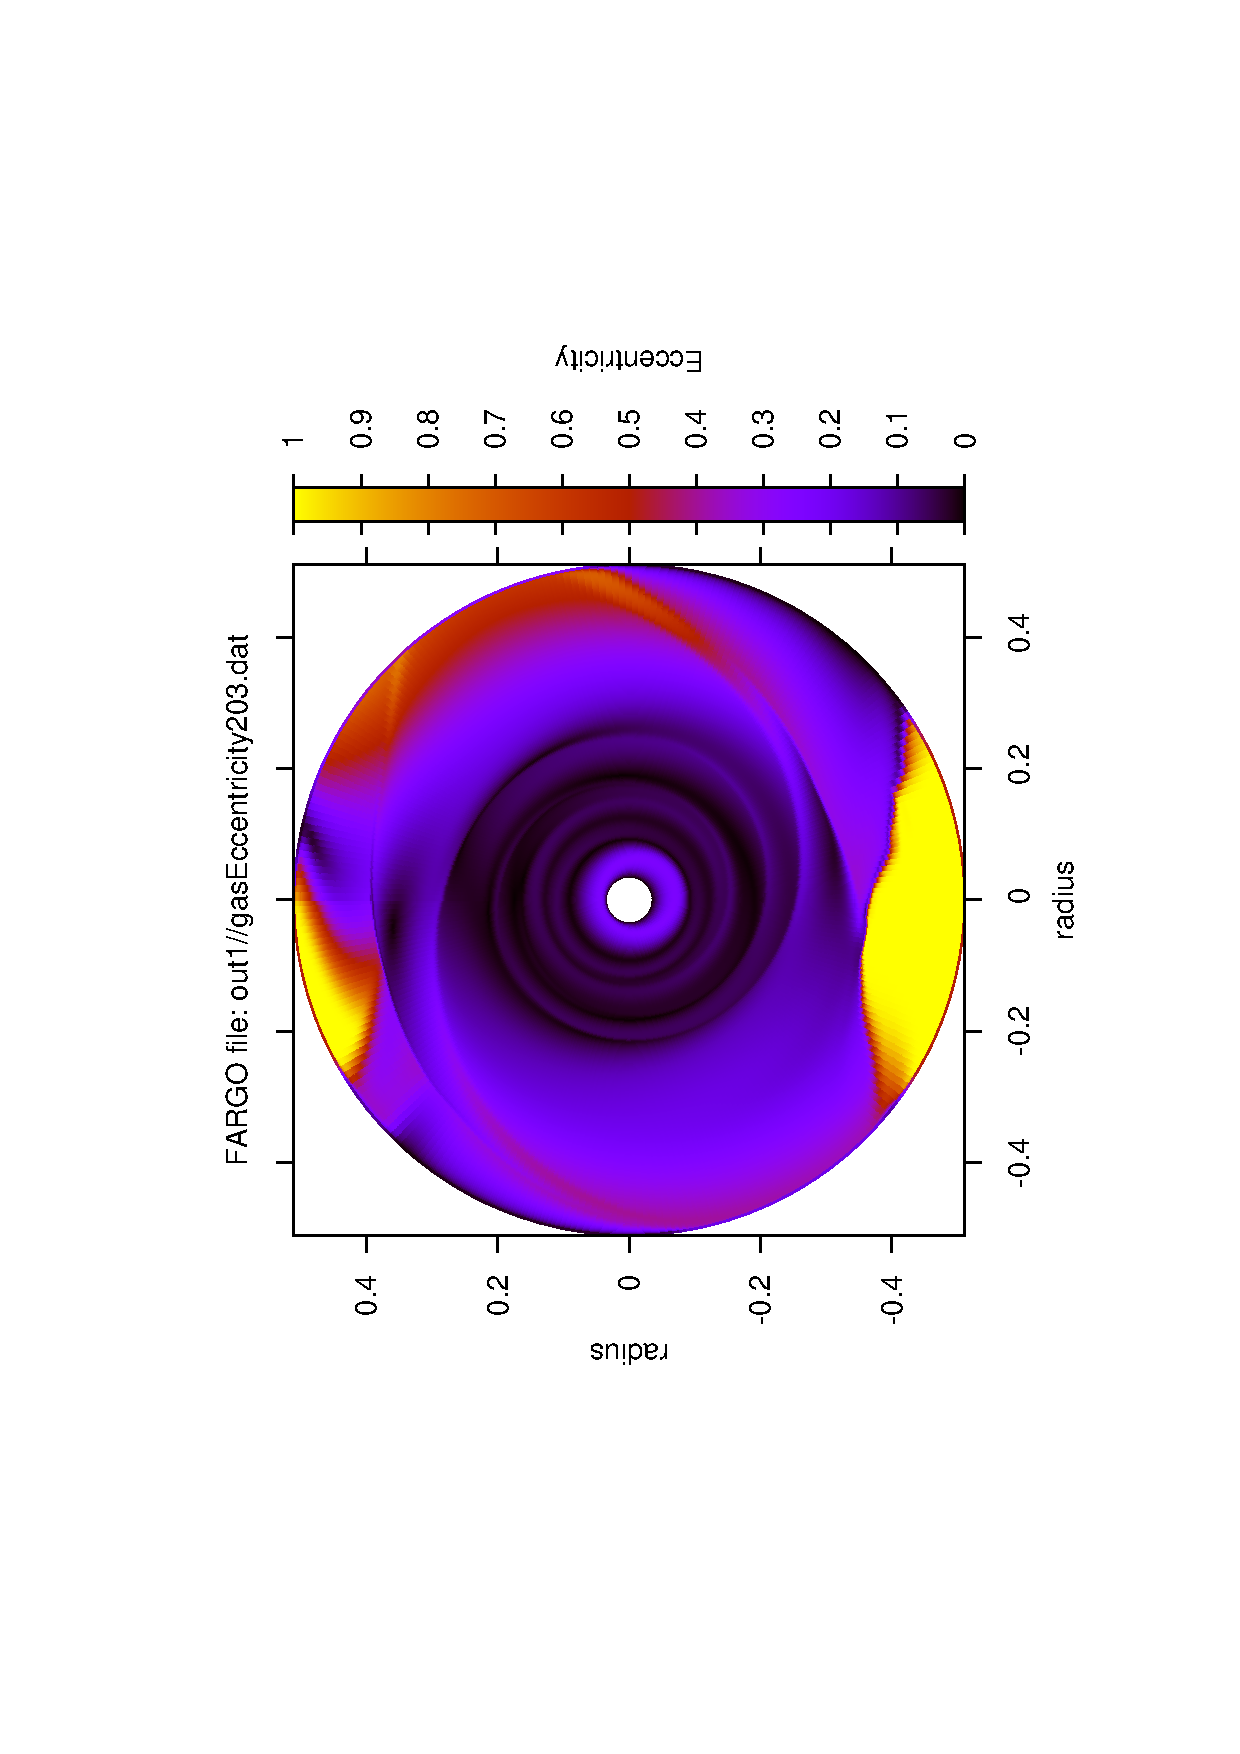
\includegraphics[scale=0.5,angle=270]{gasEccentricity203}
	\end{center}
\caption{\label{gasEccentricity203}2D-Profil der Exzentrizität einer Scheibe nach einem Binary Orbit. Wir verwenden ein $N_{\text{r}} \times N_{\varphi} = 300\times 300$ logarithmisches Gitter}
\end {figure}

\subsection{CVNR}
Der FARGO-Code hat eine künstliche Viskosität in den Druck-Quelltermen. Um einen Vergleich mit RH2D und NIRVANA durchführen zu können, kann man jetzt die künstliche Viskosität in der Variable CVNR konfigurieren. Der Standardwert ist 1.41. Wenn man Rechnungen ohne künstliche Viskosität durchführt, kommt es in der Scheibe oft zu hohen Geschwindigkeiten einzelner Zellen. Dies kann wie man in Abb. \ref{CVNRCollapse} sieht, zu einem Kollaps der Exzentrizität der Scheibe führen. Nach einer Weile erholt sich die Scheibe zwar wieder, doch macht das physikalisch einfach keinen Sinn:
\begin {figure}
	\begin{center}
		\input{CVNRCollapse}
	\end{center}
\caption{\label{CVNRCollapse}Ohne künstliche Viskosität werden Zellen am Rand der Scheibe sehr schnell und bringen die Scheibe zum kollabieren.}
\end {figure}


Wenn man dieselbe Rechnung mit CVNR = 1.41 berechnet, hat man anfangs dieselbe Steigung und den Selben Endwert, aber nicht den starken Abfall dazwischen.


\subsection{Boundary-Conditions}
FARGO hat folgende Randbedingungen implementiert:
\begin{itemize}
\item Open:
Offene Randbedingungen lassen, wie der Name schon sagt, die Materie und die damit verbundene Energie am Rand einfach ausströmen. Es ist zu beachten, dass schnell viel Materie verloren gehen kann (Abb. \ref{diskmass}). Das heisst, dass man bei langen Rechnungen überprüfen muss, ob überhaupt noch mit genug Masse gerechnet wird, um physikalisch einen Sinn zu machen und man nicht nur numerische Artefakte sieht. Die Implementierung der offenen Randbedingungen am Innenrand ist:
\begin{align}
\Sigma_{0,j} = \Sigma_{1,j}
\\
\epsilon_{0,j} = \epsilon_{1,j}
\\
v^{r}_{0,j} = v^{r}_{0,j} = \left\{\begin{array}{cc}
0 & v_{2.j}^{r} > 0\\ v_{2.j}^{r} & \text{sonst}
\end{array}
\right.\end{align}

Bei offenen Randbedingungen geht sehr viel Masse verloren:
\begin {figure}
	\begin{center}
		% GNUPLOT: LaTeX picture with Postscript
\begingroup
  \makeatletter
  \providecommand\color[2][]{%
    \GenericError{(gnuplot) \space\space\space\@spaces}{%
      Package color not loaded in conjunction with
      terminal option `colourtext'%
    }{See the gnuplot documentation for explanation.%
    }{Either use 'blacktext' in gnuplot or load the package
      color.sty in LaTeX.}%
    \renewcommand\color[2][]{}%
  }%
  \providecommand\includegraphics[2][]{%
    \GenericError{(gnuplot) \space\space\space\@spaces}{%
      Package graphicx or graphics not loaded%
    }{See the gnuplot documentation for explanation.%
    }{The gnuplot epslatex terminal needs graphicx.sty or graphics.sty.}%
    \renewcommand\includegraphics[2][]{}%
  }%
  \providecommand\rotatebox[2]{#2}%
  \@ifundefined{ifGPcolor}{%
    \newif\ifGPcolor
    \GPcolortrue
  }{}%
  \@ifundefined{ifGPblacktext}{%
    \newif\ifGPblacktext
    \GPblacktexttrue
  }{}%
  % define a \g@addto@macro without @ in the name:
  \let\gplgaddtomacro\g@addto@macro
  % define empty templates for all commands taking text:
  \gdef\gplbacktext{}%
  \gdef\gplfronttext{}%
  \makeatother
  \ifGPblacktext
    % no textcolor at all
    \def\colorrgb#1{}%
    \def\colorgray#1{}%
  \else
    % gray or color?
    \ifGPcolor
      \def\colorrgb#1{\color[rgb]{#1}}%
      \def\colorgray#1{\color[gray]{#1}}%
      \expandafter\def\csname LTw\endcsname{\color{white}}%
      \expandafter\def\csname LTb\endcsname{\color{black}}%
      \expandafter\def\csname LTa\endcsname{\color{black}}%
      \expandafter\def\csname LT0\endcsname{\color[rgb]{1,0,0}}%
      \expandafter\def\csname LT1\endcsname{\color[rgb]{0,1,0}}%
      \expandafter\def\csname LT2\endcsname{\color[rgb]{0,0,1}}%
      \expandafter\def\csname LT3\endcsname{\color[rgb]{1,0,1}}%
      \expandafter\def\csname LT4\endcsname{\color[rgb]{0,1,1}}%
      \expandafter\def\csname LT5\endcsname{\color[rgb]{1,1,0}}%
      \expandafter\def\csname LT6\endcsname{\color[rgb]{0,0,0}}%
      \expandafter\def\csname LT7\endcsname{\color[rgb]{1,0.3,0}}%
      \expandafter\def\csname LT8\endcsname{\color[rgb]{0.5,0.5,0.5}}%
    \else
      % gray
      \def\colorrgb#1{\color{black}}%
      \def\colorgray#1{\color[gray]{#1}}%
      \expandafter\def\csname LTw\endcsname{\color{white}}%
      \expandafter\def\csname LTb\endcsname{\color{black}}%
      \expandafter\def\csname LTa\endcsname{\color{black}}%
      \expandafter\def\csname LT0\endcsname{\color{black}}%
      \expandafter\def\csname LT1\endcsname{\color{black}}%
      \expandafter\def\csname LT2\endcsname{\color{black}}%
      \expandafter\def\csname LT3\endcsname{\color{black}}%
      \expandafter\def\csname LT4\endcsname{\color{black}}%
      \expandafter\def\csname LT5\endcsname{\color{black}}%
      \expandafter\def\csname LT6\endcsname{\color{black}}%
      \expandafter\def\csname LT7\endcsname{\color{black}}%
      \expandafter\def\csname LT8\endcsname{\color{black}}%
    \fi
  \fi
  \setlength{\unitlength}{0.0500bp}%
  \begin{picture}(7200.00,5040.00)%
    \gplgaddtomacro\gplbacktext{%
      \csname LTb\endcsname%
      \put(1738,704){\makebox(0,0)[r]{\strut{} 0.00075}}%
      \put(1738,1229){\makebox(0,0)[r]{\strut{} 0.0008}}%
      \put(1738,1754){\makebox(0,0)[r]{\strut{} 0.00085}}%
      \put(1738,2279){\makebox(0,0)[r]{\strut{} 0.0009}}%
      \put(1738,2805){\makebox(0,0)[r]{\strut{} 0.00095}}%
      \put(1738,3330){\makebox(0,0)[r]{\strut{} 0.001}}%
      \put(1738,3855){\makebox(0,0)[r]{\strut{} 0.00105}}%
      \put(1738,4380){\makebox(0,0)[r]{\strut{} 0.0011}}%
      \put(1870,484){\makebox(0,0){\strut{} 0}}%
      \put(2703,484){\makebox(0,0){\strut{} 1000}}%
      \put(3537,484){\makebox(0,0){\strut{} 2000}}%
      \put(4370,484){\makebox(0,0){\strut{} 3000}}%
      \put(5203,484){\makebox(0,0){\strut{} 4000}}%
      \put(6037,484){\makebox(0,0){\strut{} 5000}}%
      \put(6870,484){\makebox(0,0){\strut{} 6000}}%
      \put(440,2542){\rotatebox{90}{\makebox(0,0){\strut{}Mass [$M_{astrosun}$]}}}%
      \put(4370,154){\makebox(0,0){\strut{}Time [Years]}}%
      \put(4370,4710){\makebox(0,0){\strut{}Disk Mass}}%
    }%
    \gplgaddtomacro\gplfronttext{%
      \csname LTb\endcsname%
      \put(5883,4207){\makebox(0,0)[r]{\strut{}Mass}}%
    }%
    \gplbacktext
    \put(0,0){\includegraphics{diskmass}}%
    \gplfronttext
  \end{picture}%
\endgroup

	\end{center}
\caption{\label{diskmass}Masseverlust der Scheibe: Nach dem ersten Binärsternorbit geht der Großteil der Masse verloren: Wenn der Binärstern am nächsten ist, so ist die Wechselwirkung auch am größten. Bei längeren Rechnungen muss man beachten, dass die Scheibe nicht zu viel Masse verliert.}
\end {figure}

\item Reflecting
Bei reflektierenden Randbedingungen ist die Reflektion der Vor- und Nachteil: Zum einen verliert man weder Materie noch Energie, dafür hat man aber Reflektionen, welche zu Wellen, die sich durch die Scheibe bewegen, führen können. Die Implementierung für reflektierende Randbedingungen ist:
\begin{align}
\Sigma_{0,j} = \Sigma_{1,j}
\\
\epsilon_{0,j} = \epsilon_{1,j}
\\
v^{r}_{0,j} = v^{r}_{2,j}
\\
v^{r}_{1,j} = 0
\end{align}
\item Non-Reflecting, Evanescent haben wir nicht verwendet.
\end{itemize}
Diese Randbedingungen können jetzt getrennt für den inneren und äußeren Rand der Scheibe gesetzt werden.
\subsection{Potential-Smoothing}
Wenn sich ein Planet in der Akkretionsscheibe befindet, so wird sein Potential mit $\frac{1}{(r^2+\epsilon^2)^{\frac{1}{2}}}$ geglättet.
Wenn wir eine Akkretionsscheibe in einem Binärsternsystem betrachten, müssen wir, um sinnvolle Ergebnisse zu erhalten, den Binärstern anders betrachten als einen Planeten: Die Entfernung eines Planeten ist viel geringer. Bei Binärsternen macht also Potential-Smoothing keinen Sinn. Hier hilft man sich, indem man das Thicknesssmoothing auf z.B. $\epsilon=10^{-9}$ setzt und somit die Abfrage für das Roche-Smoothing umgeht.

\section{Modellierung exzentrischer Binärsternsysteme}
Die exzentrische Bahn des Binärsterns stört und verändert die Scheibe signifikant! Durch hohe Exzentrizitäten fliegt der Stern im Periastron sehr nah an der Scheibe vorbei und setzt sie somit bei jedem Binary Orbit grossen Kräften aus. Dies führt offensichtlich bei jedem Binary Orbit zu einer starken Änderung der Exzentrizität. Doch was passiert, wenn man sich eine größere Zeitspanne und somit mehrere Binary Orbits ansieht? Das wollen wir im Folgenden herausfinden.
\subsection{$\gamma$ Cephei}
Die erste bestätigte Entdeckung eines Exoplaneten war im Jahr 1988 von Bruce Campbell, G. A. H. Walker, und S. Yang \cite{campbellwalkeryang}. Dies war im System $\gamma$ Cephei, welches ein Binärsternsystem mit einem Unterriesen und einem Roten Zwerg ist.


Um einen Vergleich des Codes mit anderen Ergebnissen zu haben, wurde  das Setup von \cite{kley2007} gerechnet:
Physikalische Parameter:


\begin{tabular}{|c|c|c|c|c|c|c|}
\hline$M_1$ & $M_2$ & a & e & $M_p$ & $a_p$ & $e_p$\\\hline
1.59 & 0.378 & 18.5 & 0.36 & 1.70 & 2.13 & 0.20\\\hline
\end{tabular}


Diese physikalischen Parameter kann man nicht immer direkt in FARGO übertragen: FARGO verwendet als Masse für den Primärstern immer 1, also muss man die Masse des Binärsterns entsprechend skalieren: $M_1 = 1.0$; $M_2 = 0.2378$. Wir berücksichtigen hier keine Wechselwirkung des Binärsterns mit der Scheibe, d.h. der Binärstern ist auf seiner festen Bahn. Mittels der config File für die Planeten kann man auch Wechselwirkung mit der Scheibe und anderen Planeten einschalten, das ist aber noch nicht getestet worden. Genau so mit Vorsicht muss man die Code-Zeit betrachten. Nur mit dem richtigen Umrechenfaktor ergibt sich die korrekte Zeit für die Orbits. Bei einem Orbit von 1 $\unit{AU}$ und einer Gesamtmasse von 1 ist der Faktor z.B. $0.159148 = \frac{1}{2\pi}$
\begin {figure}
	\begin{center}
		\input{binstar}
	\end{center}
\caption{Der Binärstern umrundet den Primärstern auf seiner festen Umlaufbahn. Um die Fehler der Bewegung zu überprüfen, wird die zuvor angegebene Exzentrizität anhand der Bewegung berechnet.}
\end {figure}

Um erste Tests und einen Vergleich mit Kleys RH2D durchzuführen, wurde das Setup von $\gamma$ Cep verwendet. Es werden die Dichteprofile, Exzentrizitätsprofile nach einigen Binärorbits untersucht.
\begin {figure}
	\begin{center}
		% GNUPLOT: LaTeX picture with Postscript
\begingroup
  \makeatletter
  \providecommand\color[2][]{%
    \GenericError{(gnuplot) \space\space\space\@spaces}{%
      Package color not loaded in conjunction with
      terminal option `colourtext'%
    }{See the gnuplot documentation for explanation.%
    }{Either use 'blacktext' in gnuplot or load the package
      color.sty in LaTeX.}%
    \renewcommand\color[2][]{}%
  }%
  \providecommand\includegraphics[2][]{%
    \GenericError{(gnuplot) \space\space\space\@spaces}{%
      Package graphicx or graphics not loaded%
    }{See the gnuplot documentation for explanation.%
    }{The gnuplot epslatex terminal needs graphicx.sty or graphics.sty.}%
    \renewcommand\includegraphics[2][]{}%
  }%
  \providecommand\rotatebox[2]{#2}%
  \@ifundefined{ifGPcolor}{%
    \newif\ifGPcolor
    \GPcolortrue
  }{}%
  \@ifundefined{ifGPblacktext}{%
    \newif\ifGPblacktext
    \GPblacktexttrue
  }{}%
  % define a \g@addto@macro without @ in the name:
  \let\gplgaddtomacro\g@addto@macro
  % define empty templates for all commands taking text:
  \gdef\gplbacktext{}%
  \gdef\gplfronttext{}%
  \makeatother
  \ifGPblacktext
    % no textcolor at all
    \def\colorrgb#1{}%
    \def\colorgray#1{}%
  \else
    % gray or color?
    \ifGPcolor
      \def\colorrgb#1{\color[rgb]{#1}}%
      \def\colorgray#1{\color[gray]{#1}}%
      \expandafter\def\csname LTw\endcsname{\color{white}}%
      \expandafter\def\csname LTb\endcsname{\color{black}}%
      \expandafter\def\csname LTa\endcsname{\color{black}}%
      \expandafter\def\csname LT0\endcsname{\color[rgb]{1,0,0}}%
      \expandafter\def\csname LT1\endcsname{\color[rgb]{0,1,0}}%
      \expandafter\def\csname LT2\endcsname{\color[rgb]{0,0,1}}%
      \expandafter\def\csname LT3\endcsname{\color[rgb]{1,0,1}}%
      \expandafter\def\csname LT4\endcsname{\color[rgb]{0,1,1}}%
      \expandafter\def\csname LT5\endcsname{\color[rgb]{1,1,0}}%
      \expandafter\def\csname LT6\endcsname{\color[rgb]{0,0,0}}%
      \expandafter\def\csname LT7\endcsname{\color[rgb]{1,0.3,0}}%
      \expandafter\def\csname LT8\endcsname{\color[rgb]{0.5,0.5,0.5}}%
    \else
      % gray
      \def\colorrgb#1{\color{black}}%
      \def\colorgray#1{\color[gray]{#1}}%
      \expandafter\def\csname LTw\endcsname{\color{white}}%
      \expandafter\def\csname LTb\endcsname{\color{black}}%
      \expandafter\def\csname LTa\endcsname{\color{black}}%
      \expandafter\def\csname LT0\endcsname{\color{black}}%
      \expandafter\def\csname LT1\endcsname{\color{black}}%
      \expandafter\def\csname LT2\endcsname{\color{black}}%
      \expandafter\def\csname LT3\endcsname{\color{black}}%
      \expandafter\def\csname LT4\endcsname{\color{black}}%
      \expandafter\def\csname LT5\endcsname{\color{black}}%
      \expandafter\def\csname LT6\endcsname{\color{black}}%
      \expandafter\def\csname LT7\endcsname{\color{black}}%
      \expandafter\def\csname LT8\endcsname{\color{black}}%
    \fi
  \fi
  \setlength{\unitlength}{0.0500bp}%
  \begin{picture}(7200.00,5040.00)%
    \gplgaddtomacro\gplbacktext{%
      \csname LTb\endcsname%
      \put(1210,704){\makebox(0,0)[r]{\strut{} 0}}%
      \put(1210,1229){\makebox(0,0)[r]{\strut{} 100}}%
      \put(1210,1754){\makebox(0,0)[r]{\strut{} 200}}%
      \put(1210,2279){\makebox(0,0)[r]{\strut{} 300}}%
      \put(1210,2805){\makebox(0,0)[r]{\strut{} 400}}%
      \put(1210,3330){\makebox(0,0)[r]{\strut{} 500}}%
      \put(1210,3855){\makebox(0,0)[r]{\strut{} 600}}%
      \put(1210,4380){\makebox(0,0)[r]{\strut{} 700}}%
      \put(1711,484){\makebox(0,0){\strut{} 1}}%
      \put(2448,484){\makebox(0,0){\strut{} 2}}%
      \put(3185,484){\makebox(0,0){\strut{} 3}}%
      \put(3922,484){\makebox(0,0){\strut{} 4}}%
      \put(4659,484){\makebox(0,0){\strut{} 5}}%
      \put(5396,484){\makebox(0,0){\strut{} 6}}%
      \put(6133,484){\makebox(0,0){\strut{} 7}}%
      \put(6870,484){\makebox(0,0){\strut{} 8}}%
      \put(440,2542){\rotatebox{90}{\makebox(0,0){\strut{}Sigma}}}%
      \put(4106,154){\makebox(0,0){\strut{}r [AU]}}%
      \put(4106,4710){\makebox(0,0){\strut{}Density Profile in Binary Orbits}}%
    }%
    \gplgaddtomacro\gplfronttext{%
      \csname LTb\endcsname%
      \put(5883,4207){\makebox(0,0)[r]{\strut{}0 $Orb_{Bin}$}}%
      \csname LTb\endcsname%
      \put(5883,3987){\makebox(0,0)[r]{\strut{}5 $Orb_{Bin}$}}%
      \csname LTb\endcsname%
      \put(5883,3767){\makebox(0,0)[r]{\strut{}10 $Orb_{Bin}$}}%
      \csname LTb\endcsname%
      \put(5883,3547){\makebox(0,0)[r]{\strut{}15 $Orb_{Bin}$}}%
      \csname LTb\endcsname%
      \put(5883,3327){\makebox(0,0)[r]{\strut{}20 $Orb_{Bin}$}}%
      \csname LTb\endcsname%
      \put(5883,3107){\makebox(0,0)[r]{\strut{}30 $Orb_{Bin}$}}%
      \csname LTb\endcsname%
      \put(5883,2887){\makebox(0,0)[r]{\strut{}40 $Orb_{Bin}$}}%
      \csname LTb\endcsname%
      \put(5883,2667){\makebox(0,0)[r]{\strut{}60 $Orb_{Bin}$}}%
    }%
    \gplbacktext
    \put(0,0){\includegraphics{densityprofile}}%
    \gplfronttext
  \end{picture}%
\endgroup

	\end{center}
\caption{Die Entwicklung des Dichteprofils ist analog zu Kley/Nelson, die Anfangsoberflächendichte ist $\Sigma(r,\varphi) = \Sigma_0 r^{-\frac{1}{2}}$}
\end {figure}

Die zeitliche Entwicklung der Exzentrizität der Scheibe von $\gamma$ Cephei geht auch in Einklang mit Kleys Ergebnissen.

\begin {figure}
	\begin{center}
		\input{diskecccomparefargorh2d}
	\end{center}
\caption{Anfangs schwingt FARGO etwas stärker, der spätere Verlauf ist aber identisch. Die kleinen Peaks entstehen, wenn der Sekundärstern gerade im Periapsis ist, denn dann ist die Wechselwirkung am größten und somit steigt die Exzentrizität kurz an. Im Apoapsis ist dementsprechend die Wechselwirkung am niedrigsten.}
\end {figure}
 Ein weiterer Faktor ist, dass in diesem Vergleich leicht verschiedene Randbedingungen innen verwendet wurden. FARGO hat innen reflektierende, während RH2D "viscous outflow"-Bedingungen hat, also dass Material mit der lokalen, azimuthal gemittelten Geschwindigkeit durch $r_{\text{min}}$ fliessen darf. Darauf kommt man, wenn man von einer Akkretionsscheibe im Gleichgewicht ausgeht und sich den viskosen inneren Ausfluss ansieht. \cite{kley2007} verwendet.
\begin{align}
u_{\text{r}}(r_{\text{min}}) = -\frac{3}{2}\frac{\bar{\nu}}{r_{\text{min}}}
\end{align}


\section{Vergleich FARGO, NIRVANA und RH2D}
Hier wurde eine Vergleich der Entwicklung der Exzentrizität durchgeführt. Das Setup ist bei allen Rechnungen gleich:
Scheibe: h = 0.03, Inner BC: Reflecting,Outer BC: Open, $\sigma_{0}=10^{-5}$,$R_{\text{min}}=0.05, R_{\text{max}} = 0.7$ Binary Star: q = 0.1, a = 1.0, e = 0.0. 

\begin {figure}
	\begin{center}
		\input{RH2DNIRVANA}
	\end{center}
\caption{Alle 3 Codes ähneln sich bei der Exzentrizität, jedoch oszilliert FARGO nicht wie RH2D, nachdem die maximale Exzentrizität erreicht, und somit die Scheibe eingeschwungen ist. FARGO verhält sich in diesem Fall eher wie NIRVANA, auch wenn der Anstieg etwas steiler und das Maximum höher ist. Durch den exponentiellen Anstieg auf einen gewissen Wert der Exzentrizität sieht man, dass es sich um einen nichtexzentrischen Binärstern handeln muss. Wir wollen uns nun nicht-exzentrischen Binärsternsystemen widmen.}
\end {figure}

\section{Modellierung nicht-exzentrischer Binärsternsysteme: Parameterstudie: h, q}
Nun wollen wir betrachten, wie sich Scheiben verhalten, wenn der Binärstern sich auf einer Kreisbahn um die Scheibe und den Primärstern bewegt. Hier ist davon auszugehen, dass die Exzentrizität exponentiell auf einen bestimmten Wert steigt und diesen dann beibehält. Änderungen in der Langzeitentwicklung sind anders als bei exzentrischen Binärsternsystemen nur auf numerische Fehler zurückzuführen. Von einer Scheibendynamik nach Erreichen des Gleichgewichtszustandes ist nicht auzugehen.
Wir variieren die Parameter Aspectratio h = $\frac{H}{r}$, also die Dicke der Scheibe und den Parameter MassRatio q = $\frac{M_{2}}{M_{1}}$, das Massenverhältnis des Binärsterns zu dem Primärstern. 

Setup:

\begin{tabular}{|c|c|c|c|c|}
\hline$M_1 [\unit{\astrosun}]$ & $M_2$ [\unit{\astrosun}] & $\frac{H}{r}$ & a [$\unit{AU}$] & e \\\hline
1.0 & 0.1 - 1.0 & 0.03 - 0.05 & 1.0 & 0.0 \\\hline
\end{tabular}

Ziel ist es, die Wachstumsrate, sowie den Wert der Exzentrizität der Scheibe zu bestimmen. Als Randbedingungen verwenden wir innen reflektierende und außen offene.
Wir betrachten auch die Präzession der Scheibe.

Probleme traten auf, wenn die künstliche Viskosität nach von Neumann Richtmyer nicht aktiviert war. Dann werden die Berechnungszeitschritte extrem klein, die Rechnungen daürten also ewig. Dazu gibt es partiell extrem hohe Geschwindigkeiten einzelner Zellen, was zu Exzentrizitäten von weit über 1 führt. Danach kollabiert die Exzentrizität der gesamten Scheibe auf 0 und steigt langsam wieder an. Der am Ende erreichte Wert entspricht den Ergebnissen mit CVNR, jedoch ist die Growth Rate anders.

\subsubsection{Lagrange-Punkte}
Für verschiedene Massenverhältnisse des Primär- und Binär-Sterns muss man verschiedene Scheibenradien wählen, da der Maximalradius der Scheibe nur bis zu dem Lagrangepunkt $L_1$ Sinn macht. Der Lagrangepunkt $L_1$ ist der Punkt im Raum, in dem sich ein kleiner Körper (eine Zelle unserer Scheibe) im Gravitationsfeld von 2 großen Körpern (Primär- und Binärstern) in relativer Ruhe zu den beiden Körpern befindet. Bei verschiedenen Massen haben wir also verschiedene Lagrangepunkte. Der Lagrangepunkt befindet sich auf der Verbindungsgeraden des Primär- und des Binärsterns. Wir wählen als Maximalradius der Scheibe die jeweiligen Lagrangepunkte. Wenn wir die Scheibe also größer machen würden, hätten wir sofort einen grossen Masseverlust. Um das Größenverhältnis der Scheibe gleich zu halten, passen wir den Minimalradius jeder Scheibe an unser Ausgangsverhältnis von $\frac{0.7}{0.05}$ an.
\begin {figure}[!h]
	\includegraphics[scale=0.1]{2000px-Lagrange_very_massive.png}
\caption{Lagrange-Punkte: Sie lassen sich rechnerisch herleiten, wenn man die drei Massen auf einer Linie anordnet und für die Rotation um den gemeinsamen Schwerpunkt die Summe der Kräfte aus der Zentrifugalwirkung der Rotation um den gemeinsamen Schwerpunkt und aus der graviativen Anziehung untereinander zu Null setzt.}
\end {figure}
Um zu testen, inwiefern sich die Scheibendynamik verändert, wenn man die Scheibe nicht ganz bis zu dem Langrangepunkt ausdehnt, sondern etwas kleiner macht, wurde das identische Setup für zwei verschiedene Scheibengrößen : R$_{\text{1,min}}$ = 0.0395, R$_{\text{2,max}}$ = 0.5523 und R$_{\text{2,min}}$ = 0.0371, R$_{\text{2,max}}$ = 0.5194. Hier ist zu beachten, dass auch der innere Radius angepasst wurde. Dieser kleinere Radius führt zu einer leichten Verlangsamung der Berechnung, da die CFL-Bedingung bei den am nächsten zum Primärstern liegenden Zellen greift. Trotz dieser kleinen Änderung sind die Growth Rates signifikant verschieden: 0.1693 gegenüber 0.1184 bei der ca. 6 Prozent kleineren Scheibe. 
\begin {figure}[!h]
	\begin{center}
		\input{diskecclagrangecomp}
	\end{center}
\caption{Obwohl die Scheiben sich nur 6 Prozent in der Grosse unterscheiden, verhält sich die Exzentrizität sehr verschieden. Dies ist auf die nicht angepasste Scheibenmasse zurückzuführen. Diese unterscheidet sich zwar auch nur um wenige Prozent, hier sieht man aber deren Signifikanz}
\end {figure}
Was bisher aber nicht beachtet wurde, war die mit der Scheibengröße zusammenhängende Scheibenmasse bei gleicher Oberflächendichte. Da wir diese Rechnung isotherm durchführen, sollte dies keinen Unterschied machen. Trotzdem ändern wir die Oberflächendichte, um die Scheibenmasse gleich zu lassen. Dieser Test wurde für h = 0.05 und q = 0.6 gemacht. 

\begin {figure}[!h]
	\begin{center}
		\input{diskecclagrangecompsamemass}
	\end{center}
\caption{Hier ist nun die Scheibenmasse bei beiden Scheiben trotz unterschiedlicher Größe identisch: $1.53805\cdot 10^{-5}$ [Code Units]. Setup: h = 0.05, q = 0.6, R$_{\text{min}}$ = 0.0395 [$\unit{AU}$], R$_{max}$ = 0.5523 [$\unit{AU}$], Nichtexzentrischer Binärstern im Abstand von 1$\unit{AU}$ Beide Scheiben erreichen wieder nahezu die selbe Exzentrizität im Gleichgewicht}
\end {figure}

\clearpage
Wir gehen davon aus, dass diese starken Veränderungen durch die verschiedenen Innenradien der Scheiben kommen. Um dieses Verhalten weiter zu untersuchen, modifizieren wir die Aussenradien $R_{\text{max}}$ auf $R_{\text{max}}$ = 0.5 $\unit{AU}$ und $R_{\text{max}}$ = 0.6 $\unit{AU}$. Da wir uns nahe des Lagrangepunktes befinden, sollte sich in den äusseren Zellen nur noch wenig Masse befinden, die die Exzentrizität, welche durch die Masse gewichtet wird, beeinflussen kann.

\begin {figure}
	\begin{center}
		\input{diskecclagrangehighlow}
	\end{center}
\caption{Die Entwicklung der Scheibe hängt stark von dem äusseren Rand ab! Unsere Vermutung, dass nur der innere Rand relevant wäre ist falsch! Wenn die Scheibe größer ist als der Lagrangepunkt entfernt ist, fällt es weniger ins Gewicht, wie wenn die Scheibe kleiner als der Lagrangepunkt ist. Auch wenn beide Scheiben im Gleichgewicht die selbe Exzentrizität erreichen, ist der Weg dorthin sehr unterschiedlich.}
\end{figure}

\begin{tabular}{|c|c|c|}
\hline q & R$_{min}$ [$\unit{AU}$] & R$_{\text{max}}$ [$\unit{AU}$]\\\hline
0.1	& 0.05125 & 0.7175\\\hline 
0.2	& 0.0470 & 0.6585\\\hline
0.3	& 0.0443 & 0.62087\\\hline
0.4	& 0.0424 & 0.5929\\\hline
0.5	& 0.0407 & 0.5708\\\hline
0.6	& 0.0395 & 0.5523\\\hline
0.7	& 0.0383 & 0.5366\\\hline
0.8	& 0.03735 & 0.5229\\\hline
0.9	& 0.0365 & 0.5108\\\hline
1.0	& 0.0357 & 0.5\\\hline
\end{tabular}
\clearpage
\setcounter{secnumdepth}{2}
\subsubsection{Exzentrizität h = 0.05}
Die 10 Werte für h = 0.05 werden auf zwei Schaubilder aufgeteilt, um mehr erkennen zu können. Die exponentiellen Fits sind für jedes q an den Bereich, in dem die Exzentrizität steigt, angepasst.
\begin {figure}[!h]
	\begin{center}
		\input{diskeccentricityfith0052}
	\end{center}
\caption{Um das Schaubild übersichtlicher zu machen, werden nur 5 Parameter pro Schaubild dargestellt. Mit schwerer werdendem Binärstern steigt die Growth Rate an.}
\end {figure}

\begin {figure}[!h]
	\begin{center}
		\input{diskeccentricityfith005}
	\end{center}
\caption{Alle Scheiben mit h = 0.05 und größeren q haben eine ähnliche Growth Rate, jedoch benötigen sie unterschiedlich lange, um diese zu erreichen.}
\end {figure}

\begin {figure}[!h]
	\begin{center}
		% GNUPLOT: LaTeX picture with Postscript
\begingroup
  \makeatletter
  \providecommand\color[2][]{%
    \GenericError{(gnuplot) \space\space\space\@spaces}{%
      Package color not loaded in conjunction with
      terminal option `colourtext'%
    }{See the gnuplot documentation for explanation.%
    }{Either use 'blacktext' in gnuplot or load the package
      color.sty in LaTeX.}%
    \renewcommand\color[2][]{}%
  }%
  \providecommand\includegraphics[2][]{%
    \GenericError{(gnuplot) \space\space\space\@spaces}{%
      Package graphicx or graphics not loaded%
    }{See the gnuplot documentation for explanation.%
    }{The gnuplot epslatex terminal needs graphicx.sty or graphics.sty.}%
    \renewcommand\includegraphics[2][]{}%
  }%
  \providecommand\rotatebox[2]{#2}%
  \@ifundefined{ifGPcolor}{%
    \newif\ifGPcolor
    \GPcolortrue
  }{}%
  \@ifundefined{ifGPblacktext}{%
    \newif\ifGPblacktext
    \GPblacktexttrue
  }{}%
  % define a \g@addto@macro without @ in the name:
  \let\gplgaddtomacro\g@addto@macro
  % define empty templates for all commands taking text:
  \gdef\gplbacktext{}%
  \gdef\gplfronttext{}%
  \makeatother
  \ifGPblacktext
    % no textcolor at all
    \def\colorrgb#1{}%
    \def\colorgray#1{}%
  \else
    % gray or color?
    \ifGPcolor
      \def\colorrgb#1{\color[rgb]{#1}}%
      \def\colorgray#1{\color[gray]{#1}}%
      \expandafter\def\csname LTw\endcsname{\color{white}}%
      \expandafter\def\csname LTb\endcsname{\color{black}}%
      \expandafter\def\csname LTa\endcsname{\color{black}}%
      \expandafter\def\csname LT0\endcsname{\color[rgb]{1,0,0}}%
      \expandafter\def\csname LT1\endcsname{\color[rgb]{0,1,0}}%
      \expandafter\def\csname LT2\endcsname{\color[rgb]{0,0,1}}%
      \expandafter\def\csname LT3\endcsname{\color[rgb]{1,0,1}}%
      \expandafter\def\csname LT4\endcsname{\color[rgb]{0,1,1}}%
      \expandafter\def\csname LT5\endcsname{\color[rgb]{1,1,0}}%
      \expandafter\def\csname LT6\endcsname{\color[rgb]{0,0,0}}%
      \expandafter\def\csname LT7\endcsname{\color[rgb]{1,0.3,0}}%
      \expandafter\def\csname LT8\endcsname{\color[rgb]{0.5,0.5,0.5}}%
    \else
      % gray
      \def\colorrgb#1{\color{black}}%
      \def\colorgray#1{\color[gray]{#1}}%
      \expandafter\def\csname LTw\endcsname{\color{white}}%
      \expandafter\def\csname LTb\endcsname{\color{black}}%
      \expandafter\def\csname LTa\endcsname{\color{black}}%
      \expandafter\def\csname LT0\endcsname{\color{black}}%
      \expandafter\def\csname LT1\endcsname{\color{black}}%
      \expandafter\def\csname LT2\endcsname{\color{black}}%
      \expandafter\def\csname LT3\endcsname{\color{black}}%
      \expandafter\def\csname LT4\endcsname{\color{black}}%
      \expandafter\def\csname LT5\endcsname{\color{black}}%
      \expandafter\def\csname LT6\endcsname{\color{black}}%
      \expandafter\def\csname LT7\endcsname{\color{black}}%
      \expandafter\def\csname LT8\endcsname{\color{black}}%
    \fi
  \fi
  \setlength{\unitlength}{0.0500bp}%
  \begin{picture}(8640.00,4032.00)%
    \gplgaddtomacro\gplbacktext{%
      \csname LTb\endcsname%
      \put(1342,704){\makebox(0,0)[r]{\strut{} 0.03}}%
      \csname LTb\endcsname%
      \put(1342,1085){\makebox(0,0)[r]{\strut{} 0.04}}%
      \csname LTb\endcsname%
      \put(1342,1466){\makebox(0,0)[r]{\strut{} 0.05}}%
      \csname LTb\endcsname%
      \put(1342,1847){\makebox(0,0)[r]{\strut{} 0.06}}%
      \csname LTb\endcsname%
      \put(1342,2229){\makebox(0,0)[r]{\strut{} 0.07}}%
      \csname LTb\endcsname%
      \put(1342,2610){\makebox(0,0)[r]{\strut{} 0.08}}%
      \csname LTb\endcsname%
      \put(1342,2991){\makebox(0,0)[r]{\strut{} 0.09}}%
      \csname LTb\endcsname%
      \put(1342,3372){\makebox(0,0)[r]{\strut{} 0.1}}%
      \csname LTb\endcsname%
      \put(1474,484){\makebox(0,0){\strut{} 0}}%
      \csname LTb\endcsname%
      \put(2717,484){\makebox(0,0){\strut{} 0.2}}%
      \csname LTb\endcsname%
      \put(3960,484){\makebox(0,0){\strut{} 0.4}}%
      \csname LTb\endcsname%
      \put(5203,484){\makebox(0,0){\strut{} 0.6}}%
      \csname LTb\endcsname%
      \put(6446,484){\makebox(0,0){\strut{} 0.8}}%
      \csname LTb\endcsname%
      \put(7689,484){\makebox(0,0){\strut{} 1}}%
      \put(440,2038){\rotatebox{90}{\makebox(0,0){\strut{}$\sigma$}}}%
      \put(4892,154){\makebox(0,0){\strut{}q}}%
      \put(4892,3702){\makebox(0,0){\strut{}h = 0.05}}%
    }%
    \gplgaddtomacro\gplfronttext{%
      \csname LTb\endcsname%
      \put(7323,1097){\makebox(0,0)[r]{\strut{}Fit-Errors}}%
      \csname LTb\endcsname%
      \put(7323,877){\makebox(0,0)[r]{\strut{}Eccentricity}}%
    }%
    \gplbacktext
    \put(0,0){\includegraphics{diskeccentricityerrorsh005}}%
    \gplfronttext
  \end{picture}%
\endgroup

	\end{center}
\caption{Mit schwerer werdendem Binärstern steigt die Growth Rate an und hat ihr Maximum bei q$ = 0.7$. Der Bereich von q = 0.5 bis q = 1.0 hat für h = 0.05 eine sehr ähnliche Growth Rate}
\end {figure}
Die Rechnungen mit h = 0.05 liefen am problemlosesten. Da im Vorfeld mit dem FARGO-Code die meisten Rechnungen mit h = 0.05 durchgefuhert wurden und diese sich so gutmütig verhalten, wurde der Fehler bei der von Neumann-Richtmyer Viskosität in der Azimuthalgeschwindigkeitsberechnung erst so spät gefunden.
\clearpage
\subsubsection{Exzentrizität h = 0.04}

\begin {figure}[!h]
	\begin{center}
		% GNUPLOT: LaTeX picture with Postscript
\begingroup
  \makeatletter
  \providecommand\color[2][]{%
    \GenericError{(gnuplot) \space\space\space\@spaces}{%
      Package color not loaded in conjunction with
      terminal option `colourtext'%
    }{See the gnuplot documentation for explanation.%
    }{Either use 'blacktext' in gnuplot or load the package
      color.sty in LaTeX.}%
    \renewcommand\color[2][]{}%
  }%
  \providecommand\includegraphics[2][]{%
    \GenericError{(gnuplot) \space\space\space\@spaces}{%
      Package graphicx or graphics not loaded%
    }{See the gnuplot documentation for explanation.%
    }{The gnuplot epslatex terminal needs graphicx.sty or graphics.sty.}%
    \renewcommand\includegraphics[2][]{}%
  }%
  \providecommand\rotatebox[2]{#2}%
  \@ifundefined{ifGPcolor}{%
    \newif\ifGPcolor
    \GPcolortrue
  }{}%
  \@ifundefined{ifGPblacktext}{%
    \newif\ifGPblacktext
    \GPblacktexttrue
  }{}%
  % define a \g@addto@macro without @ in the name:
  \let\gplgaddtomacro\g@addto@macro
  % define empty templates for all commands taking text:
  \gdef\gplbacktext{}%
  \gdef\gplfronttext{}%
  \makeatother
  \ifGPblacktext
    % no textcolor at all
    \def\colorrgb#1{}%
    \def\colorgray#1{}%
  \else
    % gray or color?
    \ifGPcolor
      \def\colorrgb#1{\color[rgb]{#1}}%
      \def\colorgray#1{\color[gray]{#1}}%
      \expandafter\def\csname LTw\endcsname{\color{white}}%
      \expandafter\def\csname LTb\endcsname{\color{black}}%
      \expandafter\def\csname LTa\endcsname{\color{black}}%
      \expandafter\def\csname LT0\endcsname{\color[rgb]{1,0,0}}%
      \expandafter\def\csname LT1\endcsname{\color[rgb]{0,1,0}}%
      \expandafter\def\csname LT2\endcsname{\color[rgb]{0,0,1}}%
      \expandafter\def\csname LT3\endcsname{\color[rgb]{1,0,1}}%
      \expandafter\def\csname LT4\endcsname{\color[rgb]{0,1,1}}%
      \expandafter\def\csname LT5\endcsname{\color[rgb]{1,1,0}}%
      \expandafter\def\csname LT6\endcsname{\color[rgb]{0,0,0}}%
      \expandafter\def\csname LT7\endcsname{\color[rgb]{1,0.3,0}}%
      \expandafter\def\csname LT8\endcsname{\color[rgb]{0.5,0.5,0.5}}%
    \else
      % gray
      \def\colorrgb#1{\color{black}}%
      \def\colorgray#1{\color[gray]{#1}}%
      \expandafter\def\csname LTw\endcsname{\color{white}}%
      \expandafter\def\csname LTb\endcsname{\color{black}}%
      \expandafter\def\csname LTa\endcsname{\color{black}}%
      \expandafter\def\csname LT0\endcsname{\color{black}}%
      \expandafter\def\csname LT1\endcsname{\color{black}}%
      \expandafter\def\csname LT2\endcsname{\color{black}}%
      \expandafter\def\csname LT3\endcsname{\color{black}}%
      \expandafter\def\csname LT4\endcsname{\color{black}}%
      \expandafter\def\csname LT5\endcsname{\color{black}}%
      \expandafter\def\csname LT6\endcsname{\color{black}}%
      \expandafter\def\csname LT7\endcsname{\color{black}}%
      \expandafter\def\csname LT8\endcsname{\color{black}}%
    \fi
  \fi
  \setlength{\unitlength}{0.0500bp}%
  \begin{picture}(8640.00,4032.00)%
    \gplgaddtomacro\gplbacktext{%
      \csname LTb\endcsname%
      \put(2002,700){\makebox(0,0)[r]{\strut{} 0.0497871}}%
      \csname LTb\endcsname%
      \put(2002,1711){\makebox(0,0)[r]{\strut{} 0.135335}}%
      \csname LTb\endcsname%
      \put(2002,2722){\makebox(0,0)[r]{\strut{} 0.367879}}%
      \csname LTb\endcsname%
      \put(2134,484){\makebox(0,0){\strut{} 0}}%
      \csname LTb\endcsname%
      \put(3163,484){\makebox(0,0){\strut{} 10}}%
      \csname LTb\endcsname%
      \put(4193,484){\makebox(0,0){\strut{} 20}}%
      \csname LTb\endcsname%
      \put(5222,484){\makebox(0,0){\strut{} 30}}%
      \csname LTb\endcsname%
      \put(6251,484){\makebox(0,0){\strut{} 40}}%
      \csname LTb\endcsname%
      \put(7281,484){\makebox(0,0){\strut{} 50}}%
      \csname LTb\endcsname%
      \put(8310,484){\makebox(0,0){\strut{} 60}}%
      \put(440,2038){\rotatebox{90}{\makebox(0,0){\strut{}Eccentricity}}}%
      \put(5222,154){\makebox(0,0){\strut{}Time [$P_{\text{Orb}}$]}}%
      \put(5222,3702){\makebox(0,0){\strut{}h = 0.04}}%
    }%
    \gplgaddtomacro\gplfronttext{%
      \csname LTb\endcsname%
      \put(7323,1559){\makebox(0,0)[r]{\strut{}q=0.1: Fit 0.0388$\cdot \exp({0.0380x})$}}%
      \csname LTb\endcsname%
      \put(7323,1383){\makebox(0,0)[r]{\strut{}q=0.2: Fit 0.0371$\cdot \exp({0.0777x})$}}%
      \csname LTb\endcsname%
      \put(7323,1207){\makebox(0,0)[r]{\strut{}q=0.3: Fit 0.0385$\cdot \exp({0.1102x})$}}%
      \csname LTb\endcsname%
      \put(7323,1031){\makebox(0,0)[r]{\strut{}q=0.4: Fit 0.0345$\cdot \exp({0.1205x})$}}%
      \csname LTb\endcsname%
      \put(7323,855){\makebox(0,0)[r]{\strut{}q=0.5: Fit 0.0217$\cdot \exp({0.0924x})$}}%
    }%
    \gplbacktext
    \put(0,0){\includegraphics{diskeccentricityfith0042}}%
    \gplfronttext
  \end{picture}%
\endgroup

	\end{center}
\end {figure}

\begin {figure}[!h]
	\begin{center}
		\input{diskeccentricityfith004}
	\end{center}
\caption{für ein ansteigendes Massenverhältnis steigt auch die Growth Rate, allerdings ist keine Gesetzmässigkeit zu erkennen, was in den ersten Sekundärsternorbits passiert, bzw. wann der exponentielle Anstieg der Exzentrizität beginnt.}
\end {figure}

\begin {figure}[!h]
	\begin{center}
		\input{diskeccentricityerrorsh0042}
	\end{center}
\caption{Die Exzentrizität steigt am schnellsten bei q = 0.4 und q = 0.8 an. Die Growth Rate entspricht der linearen Steigung bei einem logarithmischen Plot der zeitlichen Entwicklung der Exzentrizität. Alle Growth Rates sind sehr nahe beieinander, spannend ist aber, wie unterschiedlich lange es dauert, bis die Exzentrizität ansteigt.}
\end {figure}

\subsubsection{Exzentrizität h = 0.03}
\begin {figure}[!h]
	\begin{center}
		\input{diskeccentricityh003}
	\end{center}
\caption{Hier machen exponentielle Fits keinen Sinn mehr. Eine Growth Rate für alle 10 Parameter lässt sich nicht bestimmen. Für die Parameter ab q = 0.5 ist die Scheibe nicht mal mehr wirklich exzentrisch. Woher das rührt sehen wir gleich, wenn wir uns die Entwicklung des Periastrons für den selben Aspect Ratio h = 0.03 ansehen.}
\end {figure}
\newpage
\subsection{Periastron}
Mit der Bewegung des Periastrons sieht man die Präzession der Scheibe um den Primärstern. Die Umlauffrequenz $\bar{\omega}$ ist eine charakteristische Größe der Wechselwirkung und der Anregnungsmoden.
\subsubsection{Periastron h = 0.05}

\begin {figure}[!h]
	\begin{center}
		\input{diskperih005}
	\end{center}
	\caption{Mit zunehmendem MassRatio präzediert die Scheibe schneller}
\end {figure}





\begin {figure}[!h]
	\begin{center}
		\input{diskperiastronh005q01}
	\end{center}
\caption{Bemerkenswert bei q = 0.1 ist, dass sich der Schwerpunkt der Scheibe anfangs entgegengesetzt zu dem Sekundärstern dreht.}
\end {figure}

\begin {figure}[!h]
	\begin{center}
		\input{diskperiastronh005q03}
	\end{center}
\end {figure}
\begin {figure}[!h]
	\begin{center}
		\input{diskperiastronh005q04}
	\end{center}
\end {figure}

\begin {figure}[!h]
	\begin{center}
		\input{diskperiastronh005q10}
	\end{center}
\end {figure}

\clearpage
\subsubsection{Periastron h = 0.04}
\begin {figure}[!h]
	\begin{center}
		\input{diskperih004}
	\end{center}
	\caption{Mit zunehmendem MassRatio präzediert die Scheibe schneller und hat ihr Maximum bei q = 0.7. Der stärkste Zuwachs ist allerdings gleich am Anfang von q = 0.1 auf q = 0.2.}
\end {figure}
\begin {figure}[!h]
	\begin{center}
		\input{diskperiastronh004q01}
	\end{center}
\caption{Bei q = 0.1 dauert das Erreichen der Maximalexzentrizität am längsten, so auch die Präzession der Scheibe.}
\end {figure}

\begin {figure}[!h]
	\begin{center}
		\input{diskperiastronh004q03}
	\end{center}
\end {figure}

\begin {figure}[!h]
	\begin{center}
		\input{diskperiastronh004q06}
	\end{center}
\end {figure}
\clearpage
\begin {figure}[!h]
	\begin{center}
		\input{diskperiastronh004q07}
	\end{center}
\end {figure}

\begin {figure}[!h]
	\begin{center}
		\input{diskperiastronh004q10}
	\end{center}
\end {figure}


\subsubsection{Periastron h = 0.03}
Bei einem h von 0.03 konnte nicht für alle MassRatios ein Gleichgewichtszustand der Exzentrizität erreicht werden. Ab einem Wert von q=0.5 sind die Scheiben nicht mehr exzentrisch, somit schwingt das Periastron um 0. Für kleinere Werte von q ist die Einschwingzeit recht lange, nur für q = 0.3 und q = 0.4 sieht die Kurve gut aus.


\begin {figure}[!h]
	\begin{center}
		\input{diskperiastronh003q01}
	\end{center}
\caption{Die Scheibe fängt erst ab 120 Binärorbis an zu präzedieren, hier können aber schon numerische Fehler eine Rolle spielen.}
\end {figure}
\begin {figure}[!h]
	\begin{center}
		\input{diskperiastronh003q02}
	\end{center}
\caption{Nach 100 Binärorbits beginnt die Scheibe zu präzedieren, für q = 0.3 und 0.4 geht dies in weniger als einem Viertel.}
\end {figure}

\begin {figure}
	\begin{center}
		\input{diskperiastronh003q09}
	\end{center}
\caption{Der Verlauf des Periastrons passt genau zu der Exzentrizität: für q = 0.9 sowie q = 1.0 bleibt die Exzentrizität unter 0.1 und hat anfangs auch keinen exponentiellen Anstieg.}
\end {figure}
\clearpage
\section{Zusammenfassung}
Mit FARGO lassen sich zweidimensionale Akkretionsscheiben, welche von einem Sekundärstern gestört werden mit offenen und reflektierenden Randbedingungen bei einem Aspect Ratio von h = 0.05 ohne grössere Probleme isotherm berechnen. Sobald man sich aber wirklich lange rechnet wie in \cite{marzari2009}, adiabatisch rechnet, oder die Self-Gravity aktiviert, muss man viele Faktoren beachten und braucht optimale physikalische Setups, um gute Ergebnisse zu bekommen. für FARGO spricht, dass man durch die Multiprozessoroptimierungen verhältnismässig schnell rechnen und diese Ergebnisse mit FarGnuPlot \cite{fargnuplot} visualisieren kann.

Die Ergebnisse der Modellierung exzentrischer Binärsternsysteme erweist sich als spannender, da die Wechselwirkung stärker ist, da ein exzentrischer Sekundärstern näher an der Scheibe vorbeifliegt. Dafür muss man aber länger rechnen,da sich fast nie nach kurzer Zeit ein Gleichgewicht in der Scheibe einstellt, wie es bei nicht-exzentrischen Binärsternsystemen der Fall ist.
\section{Appendix}
Vielen Dank an meinen Zimmernachbar Tobias Müller, der mir mit seiner Diplomarbeit \cite{mueller2010} sehr geholfen hat, sowie an Alexander Seizinger, Patrick Ruoff und Simeon Carstens für anregende Diskussionen in den Kaffeepausen.

\bibliographystyle{alphadin}
\bibliography{bibliography}

\end{document}

